\documentclass[11pt,a4paper]{article}
\usepackage[utf8]{inputenc}
\usepackage[spanish]{babel}
\usepackage{amsmath}
\usepackage{graphicx}
\usepackage{color}
\usepackage{amsfonts}
\usepackage{hyperref}
\usepackage{amssymb}
\begin{document}

\begin{center}

\textcolor{blue}{Universidad de Guanajuato}\\
Geometría Computacional\\
\begin{large}
Proyecto Final\\

\end{large}
Profesora: Lizárraga Morales Rocío Alfonsina\\
17/12/2020\\
\rule{70mm}{.1mm}\\
\bf{Emmanuel Alejandro Gallardo Domínguez}\\
\bf{Guadalupe Carolina Aguirre Zúñiga}\\
145884\\

\end{center}


\begin{center}

\bf{{\huge Nenúfares - Monet}}
\end{center}

\section{Resumen:}
En este proyecto se analizó una obra del reconocido pintor Claude Monet, nenúfares (o mejor conocida como Japanese Bridge) para ser reinterpretada y convertida a una pieza digital con toques de aleatoriedad y geometría computacional.
\section{Introducción}
% Contextualización de la propuesta, justificación, propuesta
	Como propuesta de proyecto se eligió la opción de reinterpretar una obra y convertirla en una obra en digital.\\
	Claude Monet fue uno de los pioneros en el impresionismo, estilo artístico que ejecutaría toda su vida. Esta obra nos llamó mucho la atención por varios motivos:	
	
	\subsection{Los colores a usar: }
		\begin{center}
			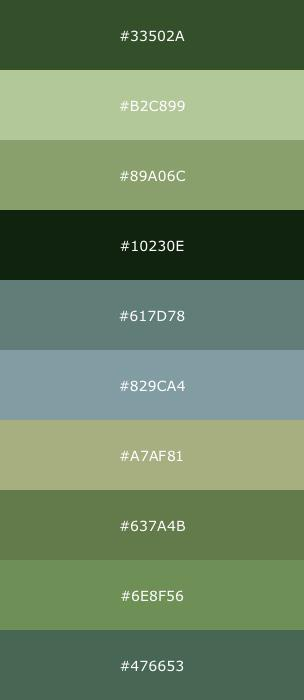
\includegraphics[scale=.3]{PaletaDeColores}
		\end{center}
			Son colores que pueden ser interpretados como "Verde, naturaleza", siempre presentes en los colores, de nuestra 	opinión, más neutrales y llamativos.
	\subsection{Los elementos que posee:}
		Al ser una representación de la naturaleza podíamos jugar con la aleatoriedad de esta, generando partes del terreno con funciones nativas de processing como veremos más adelante
	\subsection{El reto que implicaba: }
		Se asumió que la reinterpretación de una obra de impresionismo sería un buen reto técnico, por los colores, por la correcta colocación de los objetos o hasta por la programación de los mismos.

\section{Metodología}
	Para poder describir mejor el funcionamiento diseñado para este proyecto es útil dividirlo en dos diferentes tipos de módilos/objetos creados:
	\begin{itemize}
	\item {\bf Objetos:} Podemos llamarles de esta forma a los módulos que son visibles en el programa, y que si bien tienen su parte de back end al ser generados, en su mayor parte se usan como decorativos.
	\item { \bf Auxiliares: } Se trata de módulos que fueron implementados para incrementar la funcionalidad y a pesar de no ser visibles, hacen del programa cómodo de usar
	\end{itemize}
	\subsection{Objetos: }
		\subsubsection{\textcolor{blue}{Estanque}}
			
			Se trata de un objeto tridimensional que genera un mapa de ruido aleatorio usando la función \textcolor{red}{noise()} de Processing. 

			\begin{center}
			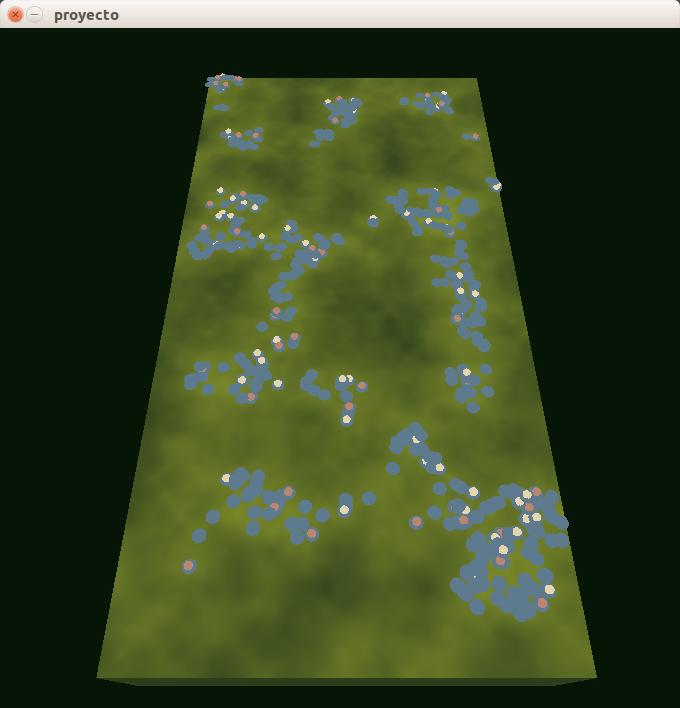
\includegraphics[scale=.5]{CAP1}
			{\tiny Estanque con mapa de ruido prueba 1}
			\end{center}
			Como se puede intuir, el mapa de ruido se genera de forma diferente cada vez que es inicializado el estanque
			\begin{center}
			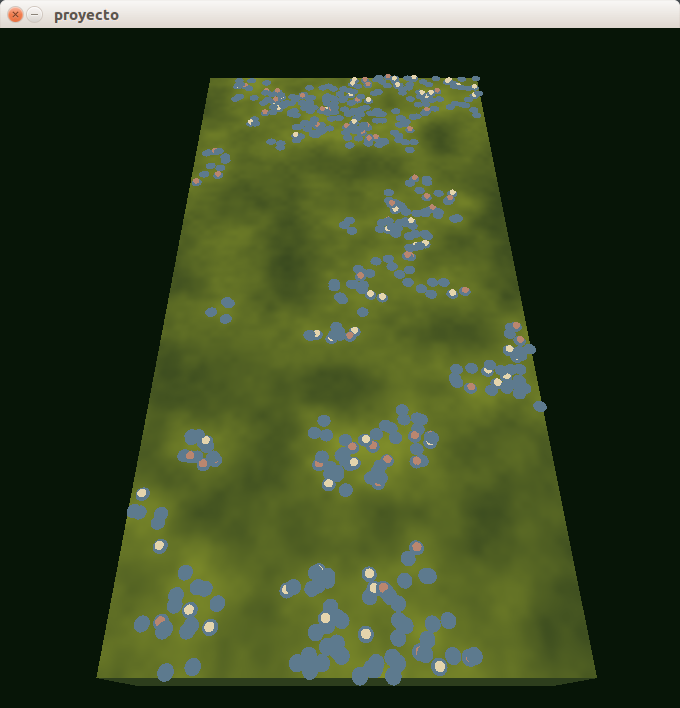
\includegraphics[scale=.5]{CAP2}
			{\tiny Estanque con mapa de ruido prueba 2}
			\end{center}

			Este mapa de ruido le indica al programa dónde puede guardar las posiciones de los nenúfares que serán generados y dibujados después.

			Con el siguiente módulo podemos generar estos:

		\subsubsection{\textcolor{blue}{Nenufar}}

			Gracias al mapa de ruido generado con el módulo anterior podemos determinar la posición en que serán dibujados los nenúfares.

			La posición de estos está guardada en un arreglo dinámico tipo \textcolor{blue}{ArrayList} nativo de processing

			Estos, dentro de sus atributos, poseen una variable tipo \textcolor{blue}{boolean} llamada \textcolor{red}{flower} la cual, si es verdadera, este poseerá una flor, la cual puede ser de dos colores distintos.

			\begin{center}
			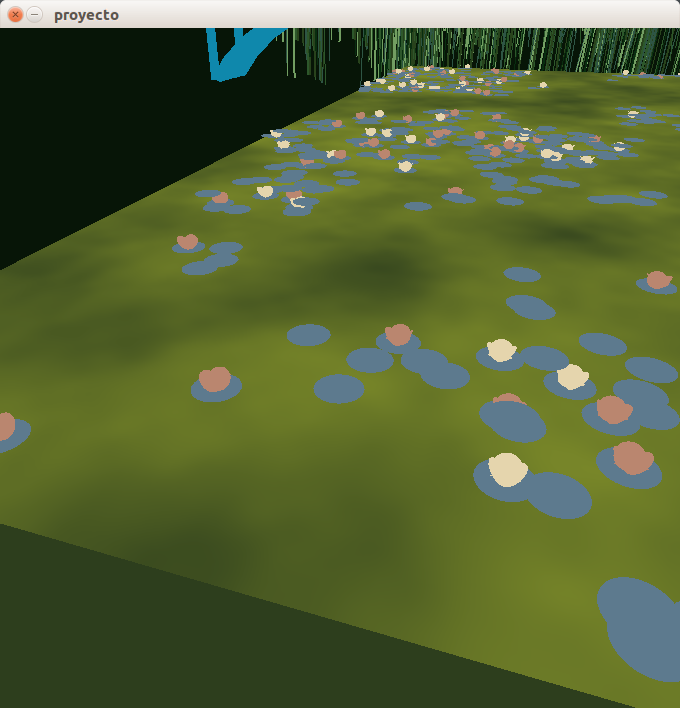
\includegraphics[scale = .5]{CAP4}\\
			{\tiny Varios nenufares, algunos con flores de distintos colores}\\
			\end{center}

			Algunas variables aleatorias de estos nenúfares están definidas desde el módulo estanque, quien es el que crea el arreglo dinámico de estos.

			\begin{center}
			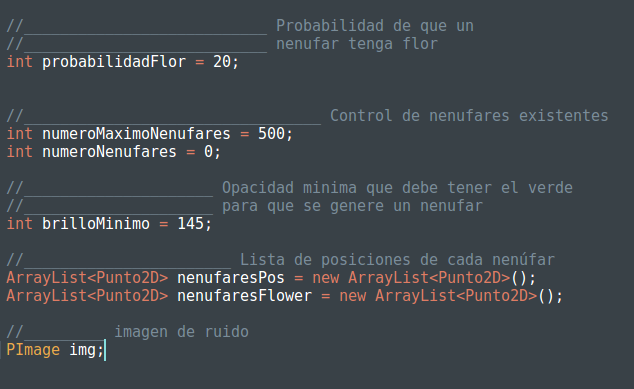
\includegraphics[scale=.5]{CAP5}\\
			{\tiny Variables aleatorias definidas desde Estanque.pde}
			\end{center}

			Para determinar las variables que serán añadidas al nenufar se usó el siguiente algoritmo:
			\begin{center}
			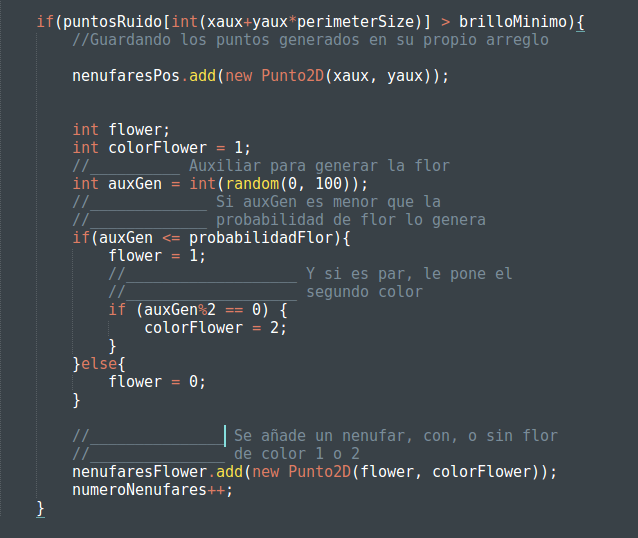
\includegraphics[scale =.5]{CAP6}
			\end{center}
		
		\subsubsection{\textcolor{blue}{Planta}}
			
			Se trata de un módulo que gestiona la manera en cómo se almacenan y dibujan ciertas hojas (pertenecientes al siguiente módulo).\\
			Las plantas, pueden ser de 4 tipos. Siendo el primero más cerrado y el último más abierto.\\
			Con su constructor se pueden establecer sus atributos, y la clase misma se encarga de generar una planta con base en estos.

			En el siguiente ejemplo se crean 4 plantas con una altura de 100, un número de 90 hojas y un tipo que se incrementa por cada número de planta, siendo la primera, de izquiera a derecha, tipo 1 y así sucesivamente.

			
			\begin{center}
			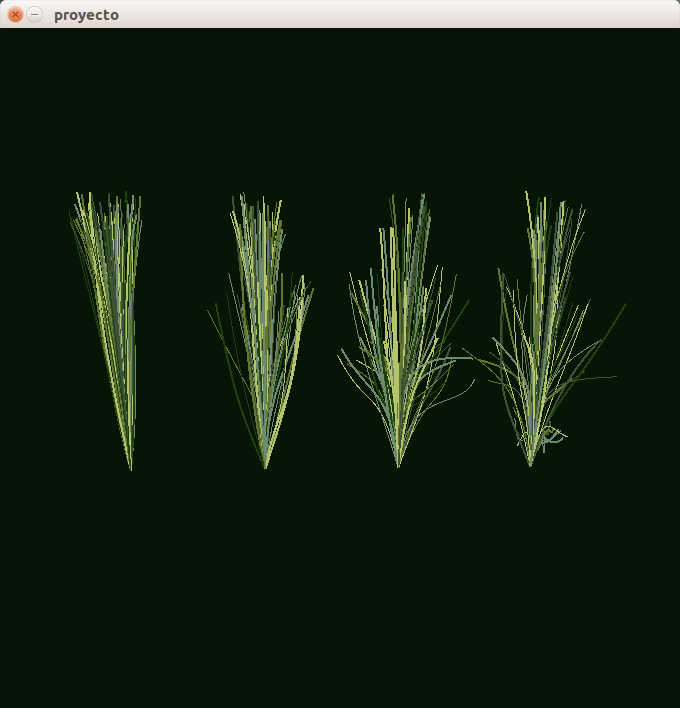
\includegraphics[scale =.4]{CAP7}
			\end{center}
			\begin{center}
			planta nuevaPlanta = \textcolor{red}{new} \textcolor{blue}{planta(altura, numeroDeHojas, Tipo)}
			\end{center}
		
		\subsubsection{\textcolor{blue}{Hoja}}

			El módulo hoja fue uno de los más complejos de diseñar, sin embargo, una vez entendida la mecánica de generación dependiendo del tipo 1, fue sencillo implementar el resto.\\
			Como explicación básica podemos resumir que:
			\begin{itemize}
				\item Se manda crear una planta
				\item El constructor crea un arreglo de hojas con los parámetros definidos
				\item Cada hoja dentro de ese arreglo se va a generar dependiendo un número aleatorio que puede estar entre el 1 (Tipo mínimo de planta) hasta el número que corresponda al tipo de planta a realizar.
			\end{itemize}
			Es decir: 
			\begin{center}
			\textcolor{blue}{El tipo de cada planta es en realidad el número máximo de tipos de hojas que tendrá dicha planta.}\\
			{\tiny Siendo el primer tipo de hoja más larga y vertical y el tipo 4 una hoja más corta y curva.}
			\end{center}
			Las plantas tipo 1 tienen su número de hojas divididas entre un solo tipo (Tipo 1)\\
			Las plantas tipo 4 tienen su número de hojas divididas entre los 4 tipos\\
			\begin{center}
			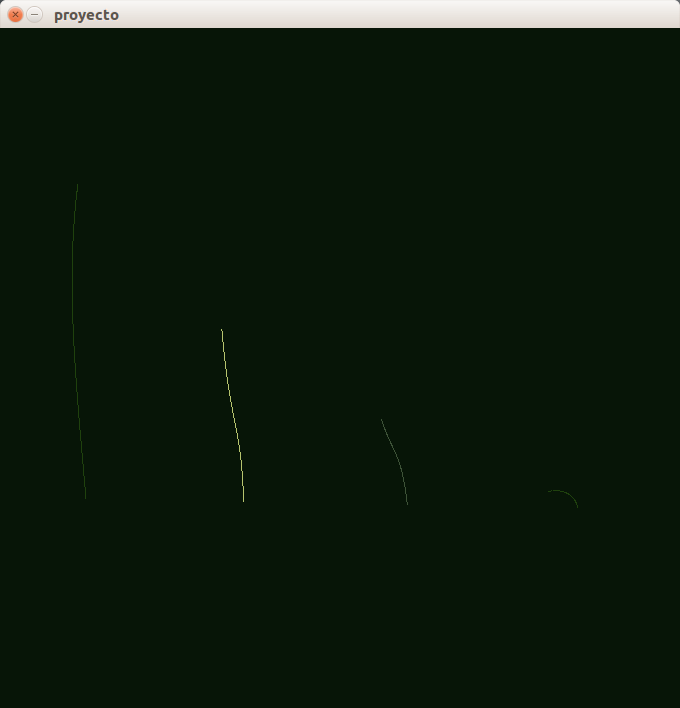
\includegraphics[scale=.4]{CAp8}\\
			{\tiny 4 hojas de 4 tipos del menor al mayor}
			\end{center}

			Así mismo, existen 4 colores disponibles para cada hoja, el cual es determinado por la probabilidad (.25)\\ 
			El objeto de hoja no es más que un conjunto de puntos en 3D los cuales son almacenados en un arreglo de tamaño 4. Los cuales al imprimirse forman una \textcolor{blue}{Curva de Bezier}. Una planta tendrá tantos arreglos de tamaño 4 como hojas tenga, y estas son dibujadas con curvas de bezier, usando sus puntos extremos como puntos finales de la curva y los dos de en medio son usados para curvar la recta formada por estos dos puntos

		\subsubsection{\textcolor{blue}{Ramal}}

			El módulo ramal es muy semejante en funcionamiento a \textcolor{blue}{planta} almacenando en su lugar objetos tipo rama y no hoja, como lo hace \textcolor{blue}{planta}

			\begin{center}
			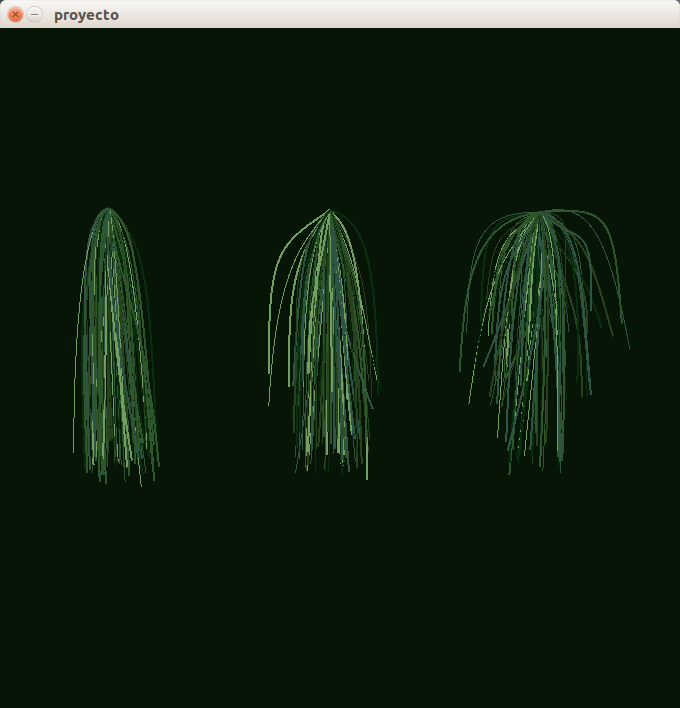
\includegraphics[scale=.4]{CAP9}\\
			{\tiny Tres tipos de ramal, del 1 al 3}
			\end{center}

		\subsubsection{\textcolor{blue}{Rama}}

			Si para el modulo planta su equivalente en inverso es rama, para la clase \textcolor{blue}{hoja} el equivalente es \textcolor{red}{rama} que usa los mismos parámetros que hoja, un arreglo de puntos en 3D que forman una \textcolor{blue}{Curva de Bezier} al ser dibujadas.

		\subsubsection{\textcolor{blue}{Puente}}

			El puente, el cual, en la obra original, representa el puente japonés que Monet tenía en su jardín de nenúfares, en esta reinterpretación fue coloreado por valores aleatorios resultando en un moderno color simulando un neón en sus respectivas variantes (verde, rojo y azul). Combinando con el perímetro de color explicado más adelante.

	\subsection{Auxiliares}

		\subsubsection{Camera}

			Para poder movernos a través del lienzo en 3D se configuraron las teclas \textcolor{blue}{W, A, S, D} para movernos hacia adelante y hacia los lados. Mientras que las teclas \textcolor{blue}{Espacio} y \textcolor{blue}{c} para subir y bajar en el espacio.\\
			Así como el mouse se usa para girar la cámara.

		 \subsubsection{Punto3D}

		 	Clase sencilla para gestionar un punto de 3 dimensiones

		 \subsubsection{Punto2D}

		 	Clase sencilla para gestionar un punto de 2 dimensiones

		 \subsubsection{Perimetro}

		 	Auxiliar que sí tiene parte gráfica, esta, además de ser auxiliar a la hora de poner los objetos en su lugar, es una rejilla decorativa generada con base a ciclos y a una distancia predeterminada.

		 	\begin{center}
		 	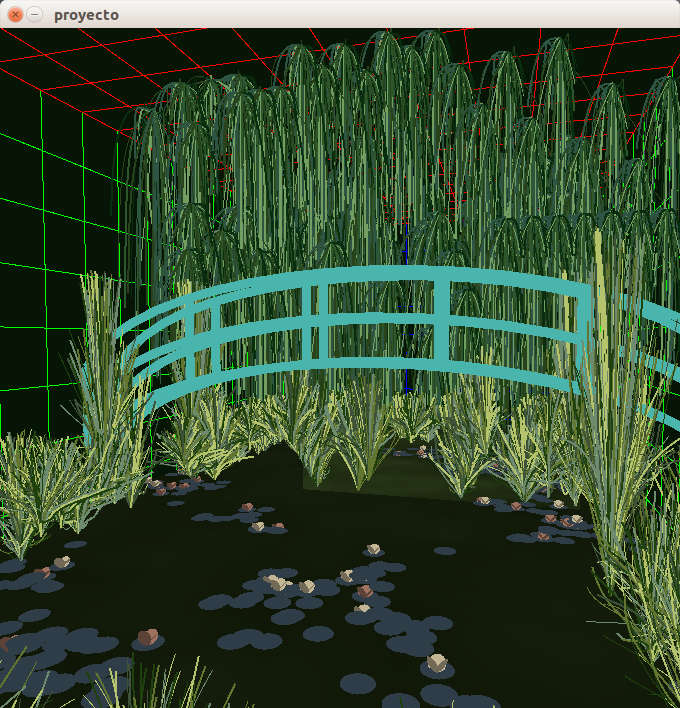
\includegraphics[scale=.5]{CAP10}\\
		 	{\tiny Imagen donde se puede apreciar todos los objetos encendidos}
		 	
		 	\end{center}

\section{Resultados}
	
		\subsection{Comparación:}
		\begin{center}
		
		\centerline{\fbox{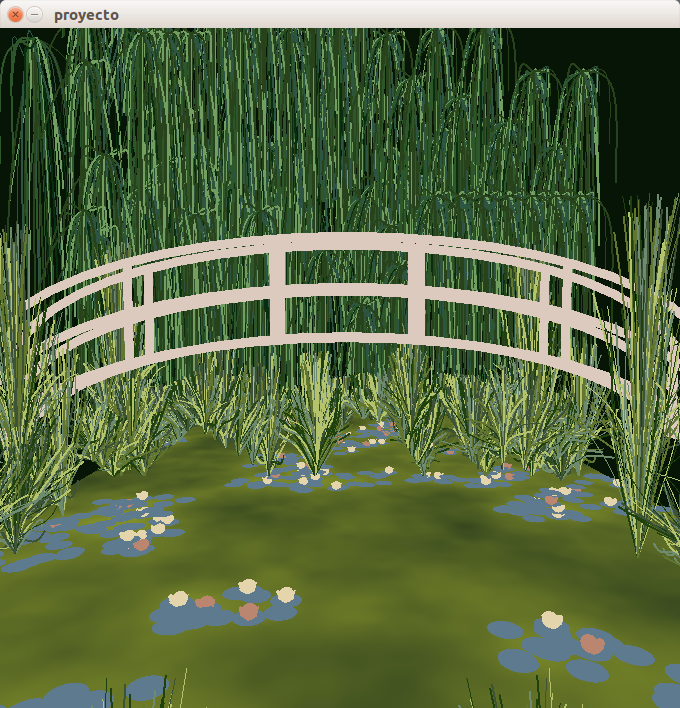
\includegraphics[scale=.32]{RES1} 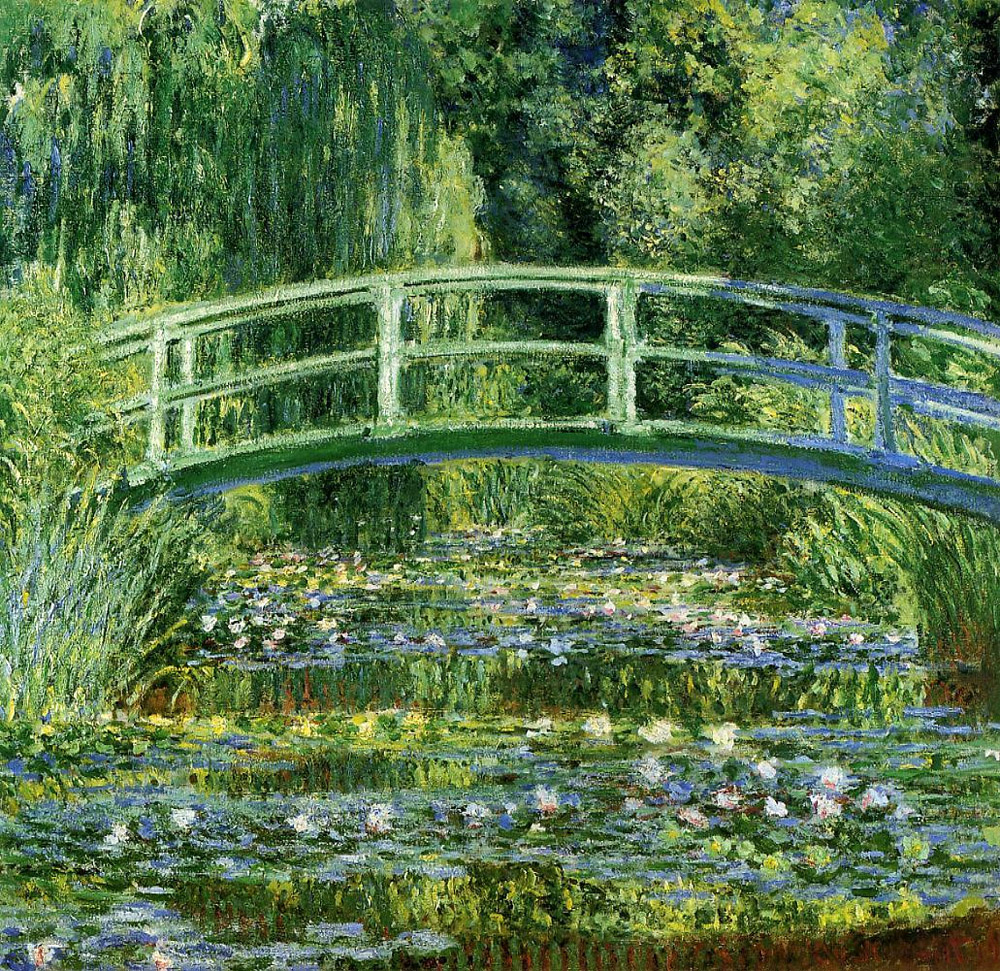
\includegraphics[scale=.22]{RES2}}}
		Reinterpretación/Original
		\end{center}

		Si bien la representación no se intentó completamente igual, sobre todo la animación que no puede ser mostrada en una sola imagen, sí se llegó a un parecido bastante notable, al menos en proporciones y distancias. Además, claro, de una interacción del usuario con la obra a través de una imersión tridimensional que se pudo lograr con la cámara.

		El código completo, así como sus commits y tiempos de elaboración se encuentra en el repositorio del administrador del proyecto:
		\begin{center}
		\fbox{\href{https://github.com/magogallardo/japaneseBridgeMonet}{\textcolor{blue}{\underline{Link del repositorio en GitHub}}}}
		
		\end{center}

		\textcolor{red}{Nota:} Debido a nuestros problemas de rendimiento, se implementó una solución temporal para poder dibujar los modelos en su correspondiente sitio, con las teclas \textcolor{blue}{R, T, Y, U, I} pueden encenderse o apagarse el estanque, las plantas, el puente, el perímetro, y los árboles, respectivamente


\section{Conclusiones}
	\textcolor{blue}{\bf Emmanuel}.- es bastante interesante la capacidad que tiene processing para gestionar figuras. Sus funciones son bastante útiles y variadas. Hasta la fecha desconozco si existen algunas que quizá me hubieran podido facilitar ciertas acciones que yo me compliqué en implementar desde cero. He de admitir que me costó algunos desvelos el encontrar la solución a ciertos problemas que me iban surgiendo, pero, advirtiendo que el código no está depurado, también sé que puede optimizarse mucho más. Nos vimos muy limitados por los recursos técnicos de nuestras computadoras, al no tener una tarjeta de video dedicada, algunas de las funciones de profundidad como las de \textcolor{blue}{hint ENABLE DEPTH SORT } el cual nos permite tener objetos sólidos, eran imposibles de ejecutar sin causar problemas mayúsculos de rendimiento. Pese a todo esto se logró un resultado positivo.
	

\section{Bibliografía}

\begin{verbatim*}

1.- https://processing.org/reference/
2.- https://es.wikipedia.org/wiki/Claude_Monet
3.- https://rtouti.github.io/graphics/perlin-noise-algorithm

\end{verbatim*}
 	
\end{document}